\documentclass[12pt]{article}
\usepackage[utf8]{inputenc}
\usepackage[margin=1in]{geometry}
\usepackage{amsfonts, amsmath, amssymb}
\usepackage[none]{hyphenat}
\usepackage{fancyhdr}
\usepackage{graphicx}
\usepackage{float}
\usepackage[nottoc, notlot, notlof]{tocbibind}
\usepackage{mathtools}
\numberwithin{equation}{section}

\pagestyle{fancy}
\fancyhead{}
\fancyfoot{}
\fancyhead[L]{\slshape \MakeUppercase{Air Column Lab}}
\fancyhead[R]{\slshape \MakeUppercase{Nenad Stoisavljević}}
\fancyfoot[C]{\thepage}
\renewcommand{\footrulewidth}{0pt}

\parindent 0ex
\renewcommand{\baselinestretch}{1.5}

\begin{document}

\begin{titlepage}
\begin{center}
\vspace*{1cm}
\Large{\textbf{John Fraser Secondary School}}\\
\Large{\textbf{Lab: Air Column}}\\
\vfill
\line(1,0){400}\\[1mm]
\huge{\textbf{Air Column Lab}}\\[3mm]
\Large{\textbf{- Air Column Lab at Home with Phyphox -}}\\[1mm]
\line(1,0){400}\\
\vfill
By Nenad Stoisavljević\\
SPH3U0-2B\\
\today\\
\end{center}
\end{titlepage}

\tableofcontents
\thispagestyle{empty}
\clearpage

\setcounter{page}{1}

\section{Phyphox}

\subsection{Observations}

\begin{itemize}
	\item Height of tube: 23.0 cm
\end{itemize}

\subsection{Screenshot of Data}

\begin{figure}[H]
	\centering
	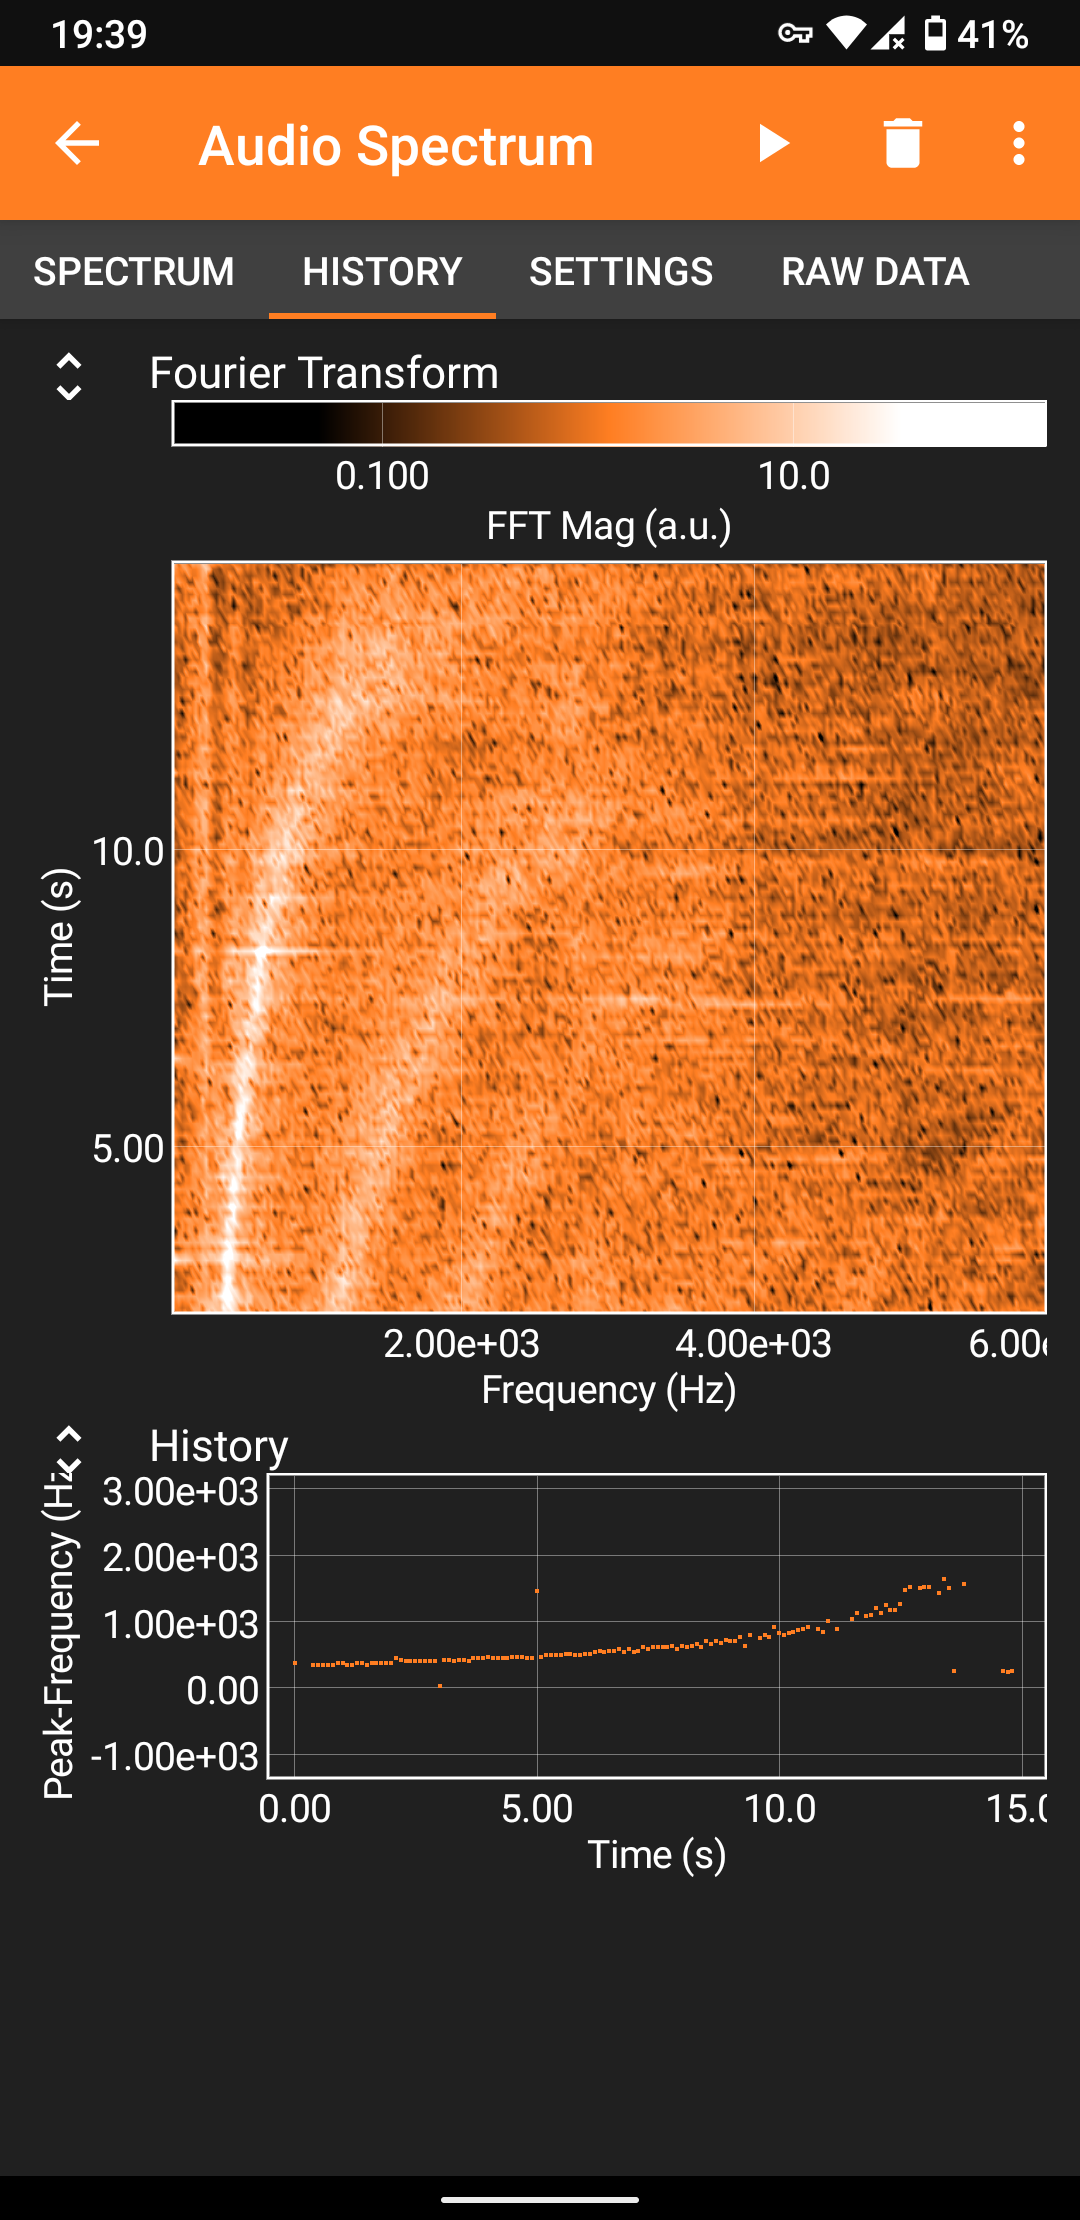
\includegraphics[scale=0.2]{data-collection/screenshot.png}
	\caption{Screenshot of Data}
	\label{fig:screenshot}
\end{figure}

\section{Analysis}

\subsection{Frequency vs. Length of Tube}

I noticed that the pitch of the sound increased as the water filled up the tube. This means that the fundamental frequency was increasing because of the rising water in the tube, this was the result of the shortening of the length. As the length of the tube decreased, the wavelength of the sound wave decreased as well because they are directly proportional.

\begin{align}
L&=0.25\lambda_{1}\\
\lambda_{1}&=4L
\end{align}

By rearranging the universal wave equation and substituting the wavelength, we can see how the length of the tube is inversely proportional to the frequency. As the length of the tube decreases, the frequency of the sound wave increases.

\begin{align}
v&=f_{1}\lambda_{1}\\
f_{1}&=\left(\frac{v}{\lambda_{1}}\right)\\
&=\left(\frac{v}{4L}\right)
\end{align}

\subsection{Peak Frequency}

The frequency of the sound wave does \textit{not} change linearly as the height of the water.

\subsection{Lower Frequency}

At 0.0 seconds, the frequency was 375.0 Hz.

\subsection{Higher Frequency}

At 13.381 seconds, the frequency was 1640.625 Hz.

\subsection{Resonant Patterns for a Closed Air Column}

\begin{figure}[H]
	\centering
	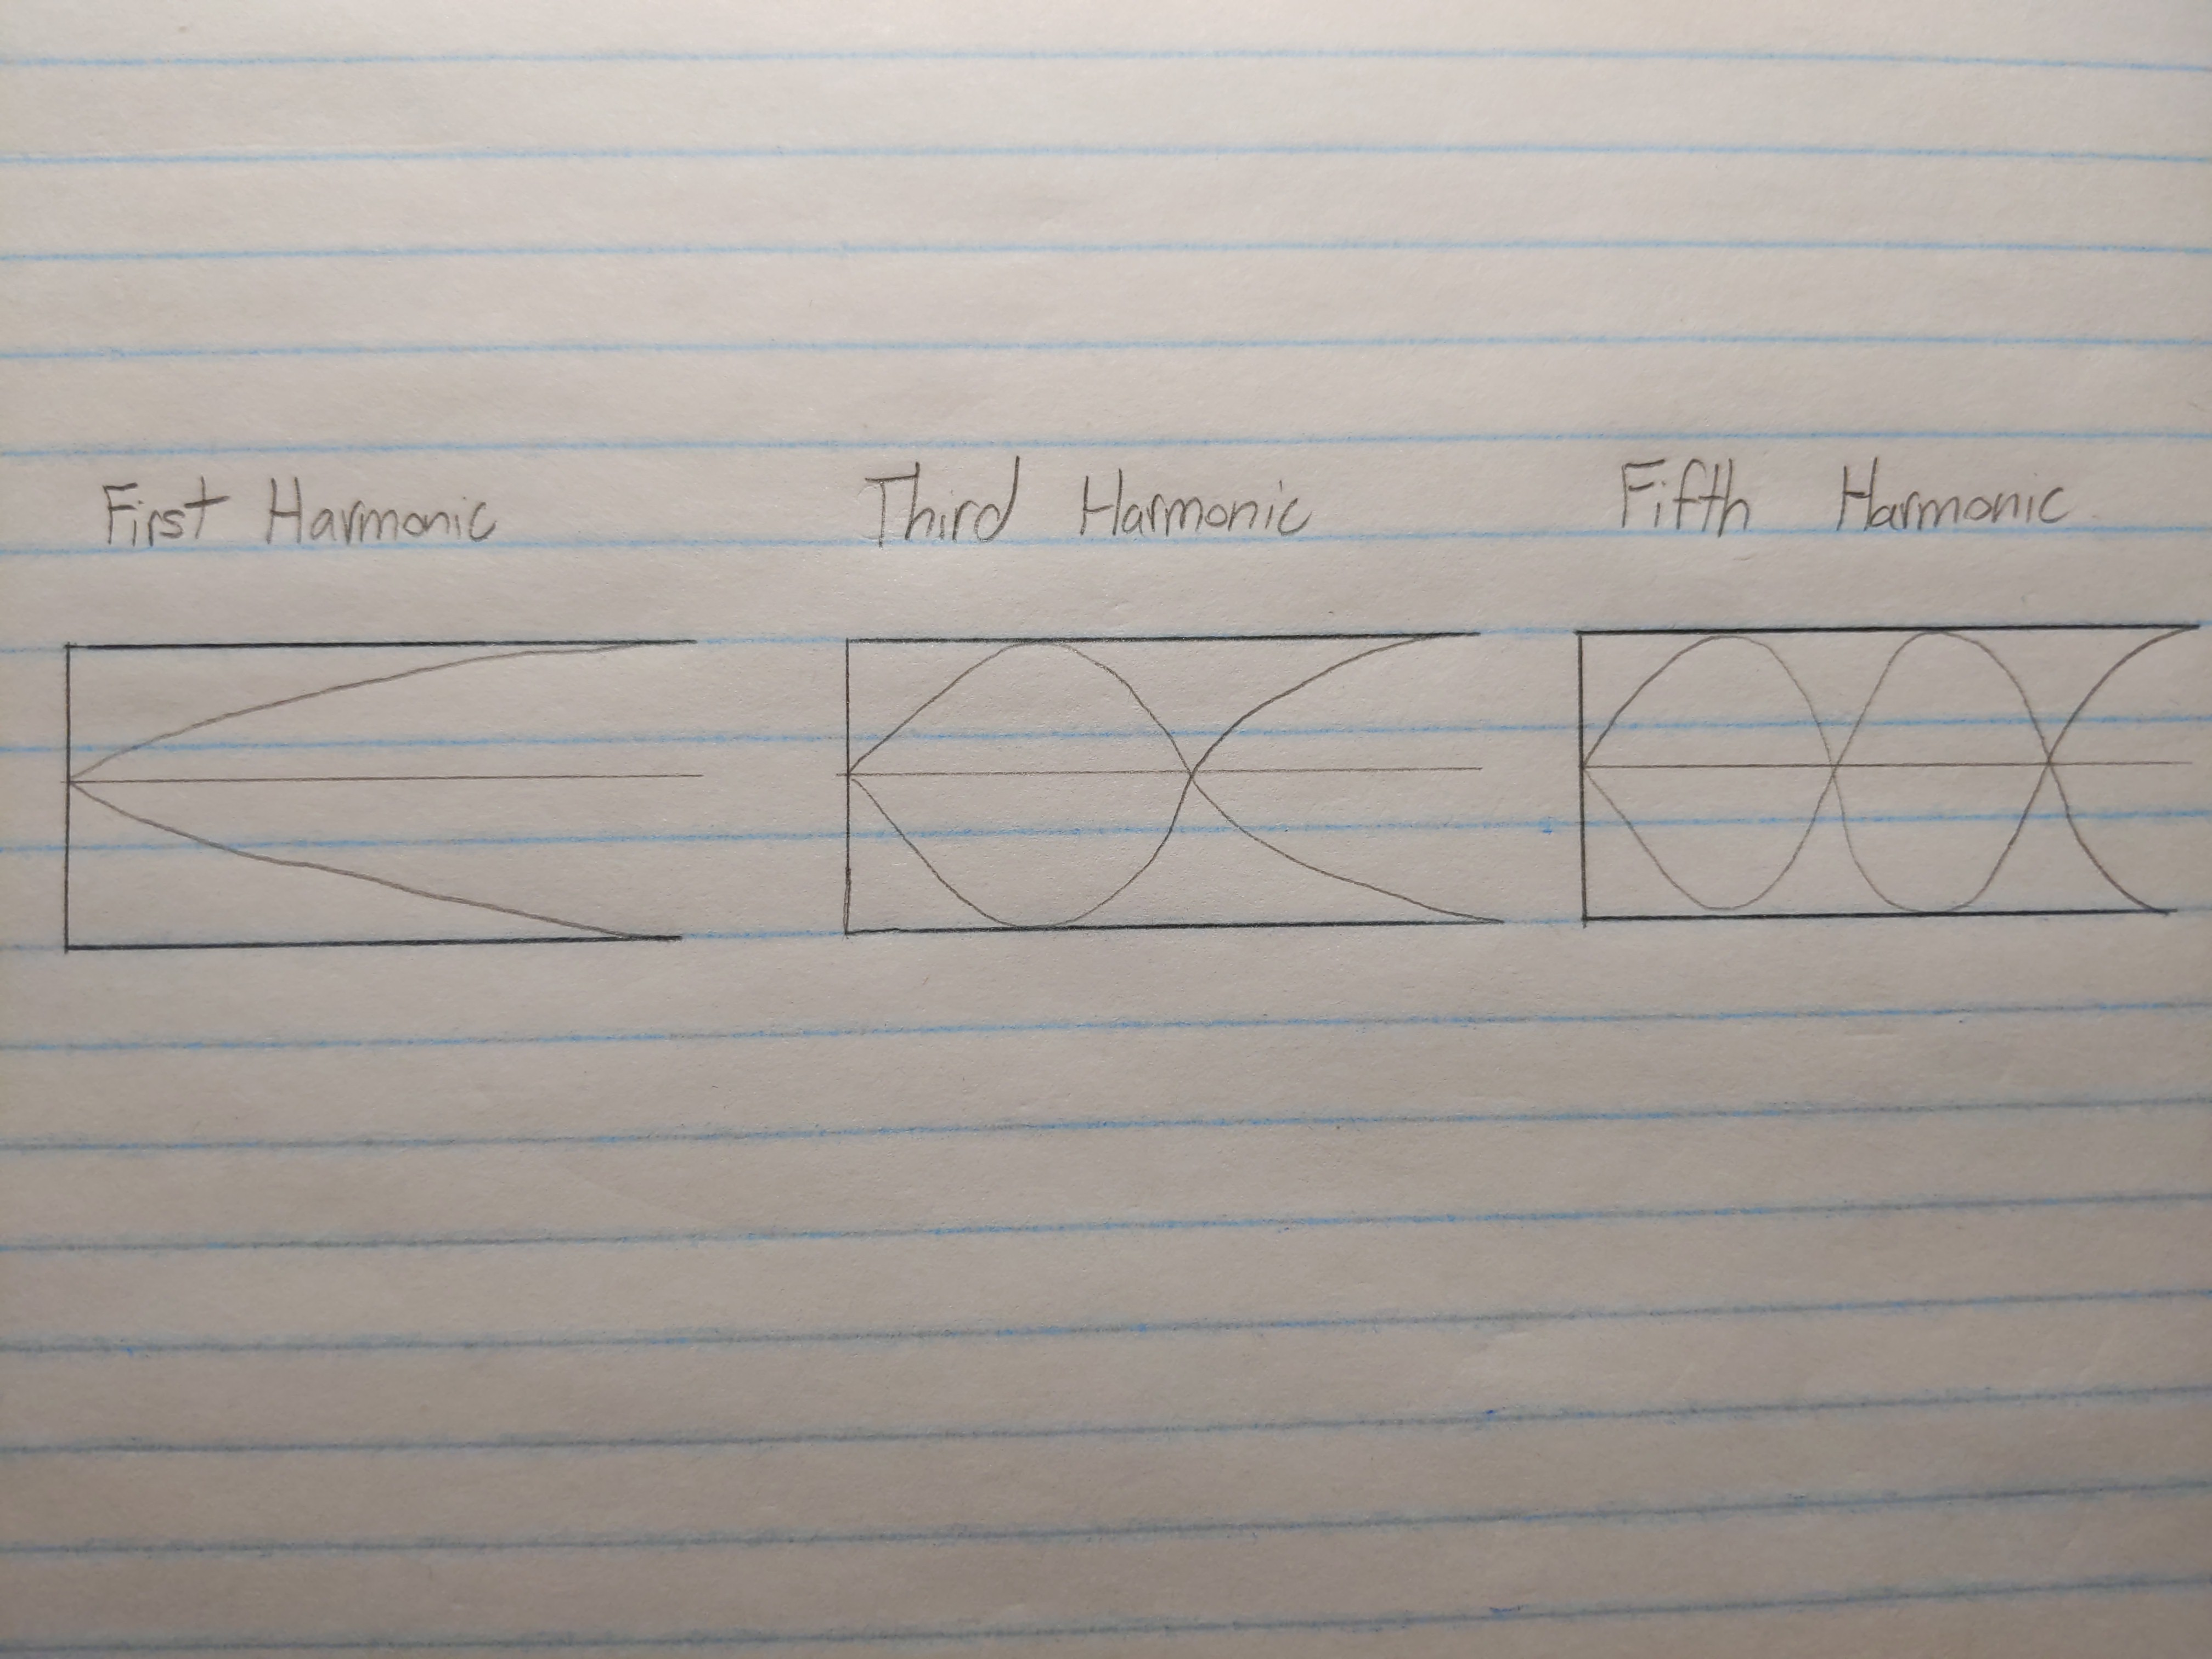
\includegraphics[scale=0.11]{data-collection/resonant-patterns.jpg}
	\caption{First Three Resonant Patterns}
	\label{fig:patterns}
\end{figure}

\subsection{Air Temperature}

Temperature: $25.0^{\circ}C$

\subsection{Speed of Sound Waves in Air}

\begin{align}
v&=331.4\,m/s+\left(\frac{0.606\,m/s}{{}^{\circ}C}\right)T\\
v&=331.4\,m/s+\left(\frac{0.606\,m/s}{{}^{\circ}C}\right)25.0^{\circ}C\\
v&=331.4\,m/s+15.15\,m/s\\
v&=346.55\,m/s\\
v&\approx347\,m/s
\end{align}

$\therefore$ the speed of sound waves in air is $347\,m/s$.

\subsection{Wavelength of the Lower Frequency Sound Wave}

It is possible for this wave to have set up a standing wave pattern because the calculations all work out. I first found out the wavelength by rearranging the universal wave equation, which gave me a value for one full wavelength.

\begin{align}
\lambda_{1}&=\frac{v}{f}_{1}\\
\lambda_{1}&=\frac{346.55\,m/s}{375.0\,Hz}\\
\lambda_{1}&=0.9241\overline{3}\,m\\
\lambda_{1}&\approx92.4\,cm
\end{align}

Now, because the tube is closed on one end and open on the other, the length of the standing wave pattern will be equal to one-fourth of the wavelength. The length of the standing wave pattern, using the calculated wavelength equates to the height of the tube, which means that it is possible for this standing wave pattern to have been set up in the air column.

\begin{align}
L&=0.25\lambda_{1}\\
L&=0.25\times0.924\,m\\
L&=0.231\,m\\
L&\approx23\,cm
\end{align}

\subsection{Wavelength of the Higher Frequency Sound Wave}

It is possible for this wave to have set up a standing wave pattern because the calculated length of the standing wave pattern is less than the height of the tube. Like before, I found the wavelength by rearranging the universal wave equation. The calculated value makes sense, because its value is lower than the wavelength with the lower frequency, as I mentioned before the wavelength and frequency are inversely proportional.

\begin{align}
\lambda_{1}&=\frac{v}{f}_{1}\\
\lambda_{1}&=\frac{346.55\,m/s}{1640.625\,Hz}\\
\lambda_{1}&\approx0.21123\,m\\
\lambda_{1}&\approx21.1\,cm
\end{align}

The calculated length is of a reasonable value, but most likely my phone stopped picking up frequencies after 5.0 cm because there should have been higher frequencies since I kept on filling up the tube with water past that length.

\begin{align}
L&=0.25\lambda_{1}\\
L&=0.25\times0.21123\,m\\
L&\approx0.0528\,m\\
L&\approx5.0\,cm
\end{align}

Using the highest frequency as the fundamental frequency, any odd number of harmonics would be possible because the length and speed of the sound wave will remain constant.

\begin{align}
f_{1}&=\frac{v}{4L}\\
f_{1}&=1640.625\,Hz
\end{align}

The number of harmonics, denoted by $f_{n}$ can be any odd number because that frequency will just be the fundamental frequency multiplied by whatever the n is.

\begin{align}
f_{n}&=n\left(\frac{v}{4L}\right)\\
f_{n}&=n\times1640.625\,Hz
\end{align}

$\therefore$ any odd number of harmonics were possible.

\subsection{Three Distinctive Curves/Trends}

I think that the three distinctive curves are indicating the first three harmonics that the microphone was picking up. Looking at the frequency axis, the three distinctive curves seem to be equally spaced apart, which most likely means that they are multiples of one another, so they must be the different harmonics or resonant patterns of the fundamental frequency.

\end{document}
